\documentclass[twoside]{article}

\usepackage{blindtext} % Package to generate dummy text throughout this template 

\usepackage[sc]{mathpazo} % Use the Palatino font
\usepackage[T1]{fontenc} % Use 8-bit encoding that has 256 glyphs
\linespread{1.05} % Line spacing - Palatino needs more space between lines
\usepackage{microtype} % Slightly tweak font spacing for aesthetics

\usepackage[english]{babel} % Language hyphenation and typographical rules

\usepackage[hmarginratio=1:1,top=32mm,columnsep=20pt]{geometry} % Document margins
\usepackage[hang, small,labelfont=bf,up,textfont=it,up]{caption} % Custom captions under/above floats in tables or figures
\usepackage{booktabs} % Horizontal rules in tables

\usepackage{lettrine} % The lettrine is the first enlarged letter at the beginning of the text

\usepackage{enumitem} % Customized lists
\setlist[itemize]{noitemsep} % Make itemize lists more compact

\usepackage{mathtools, amssymb}
\newcommand*\mean[1]{\bar{#1}}

\usepackage{caption}
\usepackage{subcaption}
\usepackage{graphicx}

\graphicspath{ {./graphics/} }

\usepackage{abstract} % Allows abstract customization
\renewcommand{\abstractnamefont}{\normalfont\bfseries} % Set the "Abstract" text to bold
\renewcommand{\abstracttextfont}{\normalfont\small\itshape} % Set the abstract itself to small italic text

\usepackage{titlesec} % Allows customization of titles
\renewcommand\thesection{\Roman{section}} % Roman numerals for the sections
\renewcommand\thesubsection{\roman{subsection}} % roman numerals for subsections
\titleformat{\section}[block]{\large\scshape\centering}{\thesection.}{1em}{} % Change the look of the section titles
\titleformat{\subsection}[block]{\large}{\thesubsection.}{1em}{} % Change the look of the section titles

\usepackage{fancyhdr} % Headers and footers
\pagestyle{fancy} % All pages have headers and footers
\fancyhead{} % Blank out the default header
\fancyfoot{} % Blank out the default footer
\fancyhead[C]{Running title $\bullet$ May 2016 $\bullet$ Vol. XXI, No. 1} % Custom header text
\fancyfoot[RO,LE]{\thepage} % Custom footer text

\usepackage{titling} % Customizing the title section

\usepackage{hyperref} % For hyperlinks in the PDF
\setlength{\droptitle}{-4\baselineskip} % Move the title up

\pretitle{\begin{center}\Huge\bfseries} % Article title formatting
\posttitle{\end{center}} % Article title closing formatting
\title{Random Forest vs. Gradient Boosting for monocular scale} % Article title
\author{%
\textsc{Alex Kreimer}\thanks{A thank you or further information} \\[1ex] % Your name
\normalsize Technion \\ % Your institution
\normalsize \href{mailto:alex.kreimer@gmail.com}{alex.kreimer@gmail.com} % Your email address
%\and % Uncomment if 2 authors are required, duplicate these 4 lines if more
%\textsc{Jane Smith}\thanks{Corresponding author} \\[1ex] % Second author's name
%\normalsize University of Utah \\ % Second author's institution
%\normalsize \href{mailto:jane@smith.com}{jane@smith.com} % Second author's email address
}
\date{\today} % Leave empty to omit a date
\renewcommand{\maketitlehookd}{%
\begin{abstract}
\noindent This works compares random forest to gradient bosting.  It does so in context of monocular scale estimation problem.
\end{abstract}
}

\begin{document}

% Print the title
\maketitle

\section{Introduction}
Recovering camera 6-DOF ego-motion from images is a well studied
problem. It arises in various practical contexts
(e.g. virtual/augmented reality application, autonomous or aided
navigation, etc.).  The problem was studied in both stereo and the
monocular setups.  To recover the full 6-DOF motion, the previous
works resorted to the stereo setup, used auxiliary sensors (e.g. IMU)
or rely on the planar motion assumption.  All of these have their
drawbacks: stereo pairs are fragile and require careful calibration
procedures, additional sensors are not always available and also
require calibration, scene assumptions don't always hold.  Motion
estimation from images of a single moving camera is probably the
hardest setup, as well as the most desirable one, because of its
simplicity.  It is well known that the translation scale parameter is
not directly observable for a motion of a single camera.

We argue, that for natural scenes the scale information is present in
the images.  We propose to apply statistical machine learning
techniques to learn the monocular scale.  In the following sections we
present an overview of the existing works in the field, describe our
method and present the experimental results.

\section{Methods}
\subsection{Our method}\label{sec:our method}

We assume that a single camera moves through space and takes images.
We treat the initial camera pose (at time $t=0$) as the world
coordinate frame.  We denote the pose of the camera at time $t$ by
$\mathbf{\hat{T}}_t$ described by the rotation matrix
$\mathbf{\hat{R}}_t$ and the translation vector $\mathbf{\hat{t}}_t$
as seen in the world coordinate frame.  We denote camera image taken
at time $t$ by $I_t$.  To facilitate the discussion, we also introduce
notation for camera pose
$\mathbf{T}_t = [\mathbf{R}_t\ |\ \mathbf{t}_t] $ as seen from the
coordinate frame associated with camera pose at time $t-1$.  Most of
the time, we will omit the time index, since its clear from the
context.  By translation scale (or simply, scale) we refer to the norm
of the translation vector $\mathbf{t}$ (e.g.,
$s = \lVert \mathbf{t} \rVert$)

We pose the scale estimation problem as a regression problem and
search for a good regressor model.

\section{Random forest}

\subsection{Decision trees}

In this section we briefly describe tree-based methods for regression.
These involve splitting the feature space into a number of small
regions.  The prediction for a sample is made by computing a mean or a
mode of training samples that belong to the same region.  Since the
set of rules used to split the feature space into smaller regions may
be described by a tree, these methods are referred to as
\textit{decision tree} methods.

Building a decision tree may be described by a two step procedure:
\begin{enumerate}
\item Split the feature space, e.g., the set of all possible values
  for $X_1, X_2,\ldots,X_n$ into $J$ distinct regions $R_1, R_2,\ldots, R_J$.
\item For every sample that belongs to the regions $R_i$ we make the
  same prediction, which is a mean of the responses of training
  samples that belong to this region.
\end{enumerate}

The regions $R_i$ are usually chosen to be multidimensional boxes (axis aligned).  We would like to find such a partition of the feature space that minimizes
\begin{equation}\label{eq:tree_objective}
\sum\limits_{j=1}^J\sum_{x\in R_j}{(x-\mean{y}_j)^2}
\end{equation}

Where $y_j$ denotes the mean of the response values of the samples in
region $R_j$.  Unfortunately, solving the optimization
problem~\ref{eq:tree_objective} is computationally hard.  Usually it
is replaced with a greedy algorithm, called \textit{recursive binary
  splitting}.  This approach starts at the top of the tree and
greedily chooses the best split at that point that minimizes the
variance of its sub-trees.  To be more precise, for each $j$ and $s$
we define the hyper-planes:

\begin{equation}
  R_1(j,s) = \{ X\lvert X_j<s \}\quad\text{and}\quad R_2(j,s) = \{ X\lvert X_j \geq s \},
\end{equation}

We seek such $j$ and $s$ that minimize the equation:

\begin{equation}
  \sum\limits_{i:x_i\in R_1(j,s)}{(x_i-y_{R_1})}^2 + \sum\limits_{i:x_i\in R_2(j,s)}{(x_i-y_{R_2})}^2,
\end{equation}

Where $y_{R_1}, y_{R_2}$ are the average responses of the samples in
$R_1(j,s), R_2(j,s)$ respectively.  Once we found the $j$ and $s$ we
recursively split each sub-tree in a similar manner.  The process is
repeated until a stopping criterion (e.g., number of nodes in the
leaf) is reached.

\subsection{Bagging}
Decision trees tend to suffer from \textit{high variance}. This means
that if we split the training set into a number of random subsets and
fit random tree into each sub-sample, we would likely to get much
different answers from these trees when asked the same question.  It
is known that the variance of a mean of a set of independent random
variables is $\frac{1}{n}$.  Thus, in order to improve the variance of
the estimator, it is possible to fit $n$ estimators, each to its
training-set and the average their predictions.  Since, usually, we
don't have $n$ training sets, we would use \textit{bootstrapping}
(e.g., sample independently with replacement from the data set).

\subsection{Random Forest}
The random forest suggests an additional improvement over bagging, by
decorrelating the random trees.  The issue they attempt to address is
this: lets say there is a very dominant feature w.r.t. to task at hand
for a given data-set.  Bagging ensures that we use different training
sets, but yet, most trees will tend to first split on this dominant
feature.  In this case the trees will resemble each other.  In random
forest, the trees are constructed by using only a subset of features
(e.g., $m = \sqrt{p}$).  This means that at calculating the splits,
the algorithm is allowed to consider only a subset of features.

\section{Gradient Boosting}

Boosting as a paradigm is one of the most powerful ideas in modern
machine learning.  The motivation for boosting was a procedure that
combines the outputs of many ``weak'' models to produce a powerful
one.  The idea of boosting was introduced in~\cite{} by means of
``AdaBoost.M1'' algorithm.  A weak model is such that performs
slightly better than random guessing.

Later works showed that AdaBoost is a way of fitting an additive
expansion in a set of elementary ``basis'' functions $G_m(x)$ (e.g.,
random trees in our case):

\begin{equation}
  f(x) = \sum_{m=1}^M\beta_m b(x;\gamma_m)
\end{equation}
where $\beta_m, m=1...M$ are the expansion coefficients, and
$b(x;\gamma)$ are simple basis functions parameterized by $\gamma$.

Typically, such model may be fit by minimizing a loss function
averaged over a training data:
\begin{equation}\label{eq:additive_model_ERM}
  \underset{\{\beta_m,\lambda_m\}}{\text{min}} \sum_{i=1}^{N}L(y_i,\sum_{m=1}^M \beta_m b(x_i;\lambda_m))
\end{equation}

Eq.~\ref{eq:additive_model_ERM} is hard to solve.  One may solve a greedy approximation instead:

\begin{equation}
  (\beta_m,G_m) = \underset{\beta,G} \sum_{i=1}^N L(y_i, f_{m-1}(x_i) + \beta G(x_i))
\end{equation}

For squared loss
\begin{equation}
  L(y, f(x)) = (y-f(x))^2
\end{equation}
one has
\begin{equation}
  L (y_i, f_{m-1}(x_i)+\beta b(x_i;\lambda)) = (y_i - f_{m-1}(x_i)-\beta b(x_i;\lambda))^2 =  (r_i - \beta b(x_i;\lambda))^2
\end{equation}
where $r_i=y_i-f_{m-1}(x_i)$ is a residual of the current model on the
$i$th observation.  Thus, for squared loss, the term that best fits
the current residuals is added to the expansion at each step.

\section{Experiments}
\subsection{Data-set}

We train and test on the KITTI data-set~\cite{geiger2013vision}.  The
data-set consists of 11 sequences with ground truth data.  We
arbitrarily use sequence 00 for testing and sequences 01-10 for
training.  There are 4540 and 14950 images in the test and the train
sets respectively. We only use the data from the left color camera.

\subsection{Features}\label{sec:features}

Training a random forest or gradient boosting regressor requires hand
crafted feature extraction.  We convert subsequent image pairs to
feature vectors as follows: we extract and match sparse salient points
in both input images.  The output of this stage is a set of a
corresponding pixel locations.  For each salient feature we compute
the spacial displacement magnitudes (e.g., sparse optical flow).  We
define a grid in the image space and assign each salient point to a
bin.  Next, we create histogram of displacement magnitudes for each
bin.  Concatenating all histograms together produces a feature
vector. We use Harris corners and square $11\times 11$ patches as
corner descriptors. Sum of square differences is used as a distance
measure with the winning pair declared a match.  To prune the outliers
we fit the fundamental matrix into the matched corner sets and remove
the corners that do not agree with the model.

One of the goals of this project is to do parameter search for feature
extraction. We bin each image into $n_x\times x_y$ grid:
$n_x=3\ldots 8$, $n_y=2\ldots 5$.  For each bin in the image we
compute the histogram of corner disparities.  By disparity we denote
the displacement of the corner in the image.  We use $n_{bins}$-bin
histogram for disparities: $n_{bins}=100\ldots 900$ (e.g., feature
vector length is $n_x \times n_y \times n_{bins}$).

We use these feature vectors to fit both random forest and gradient
boosted tree regressors.  We use scikit-lean~\cite{scikit-learn}
random forest implementation and XGBoost~\cite{2016arXiv160302754C}
boosted trees implementation.

\section{Results}

This sections presents results of our experiments.  We report average
mean error over the test sequence as a metric for regressor
performance.  Given a sequence of $N$ predicted motion scales
$\{\hat{y}\}_{i=1}^N$ and a corresponding sequence of the ground truth
scales $\{y\}_{i=1}^N$, we report the following loss:
\begin{equation}
  \mu = \frac{1}{N}\sum_{i=1}^N |\hat{y} - y|,
\end{equation}

Figures~\ref{fig:rf_loss_over_bins}, ~\ref{fig:xgb_loss_over_bins}
show losses as a function of the histogram size ($n_{bins}$) for the
random forest and the gradient boosting.  Every dot in a graph
corresponds to some specific model (i.e., a specific set of
$n_x, n_y, n_bins$) out of 240 possible combinations we search over.
\begin{figure}[!ht]
  \centering
  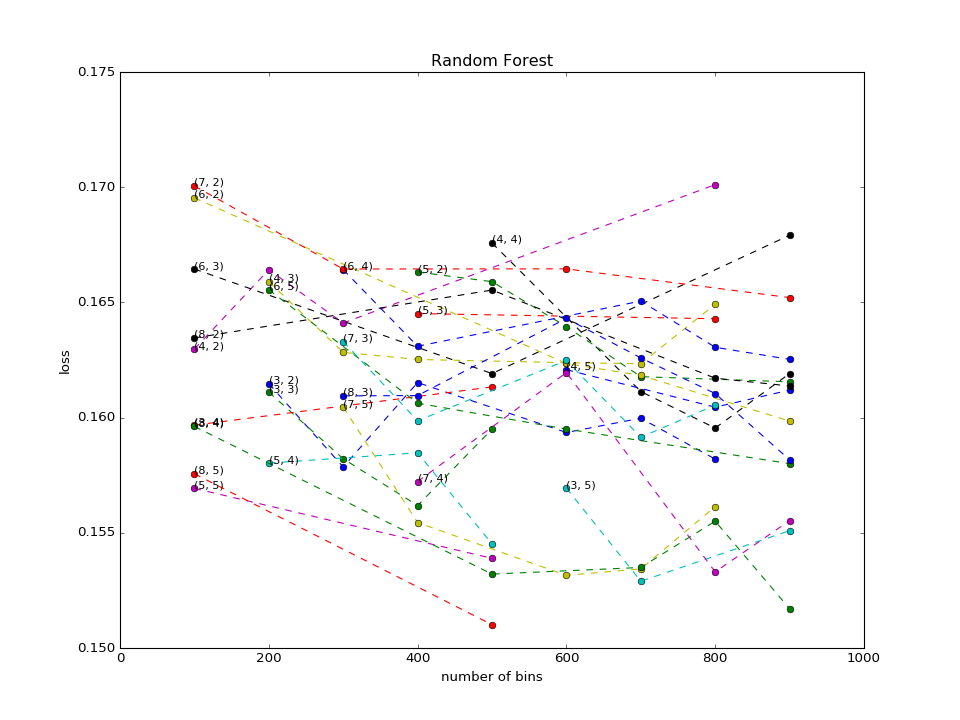
\includegraphics[width=0.6\linewidth]{rf_loss_over_bins}
  \caption{Random Forest average test sequence error as a function of $\protect n_{bins}$ }
  \label{fig:rf_loss_over_bins}
\end{figure}

\begin{figure}[!ht]
  \centering  
  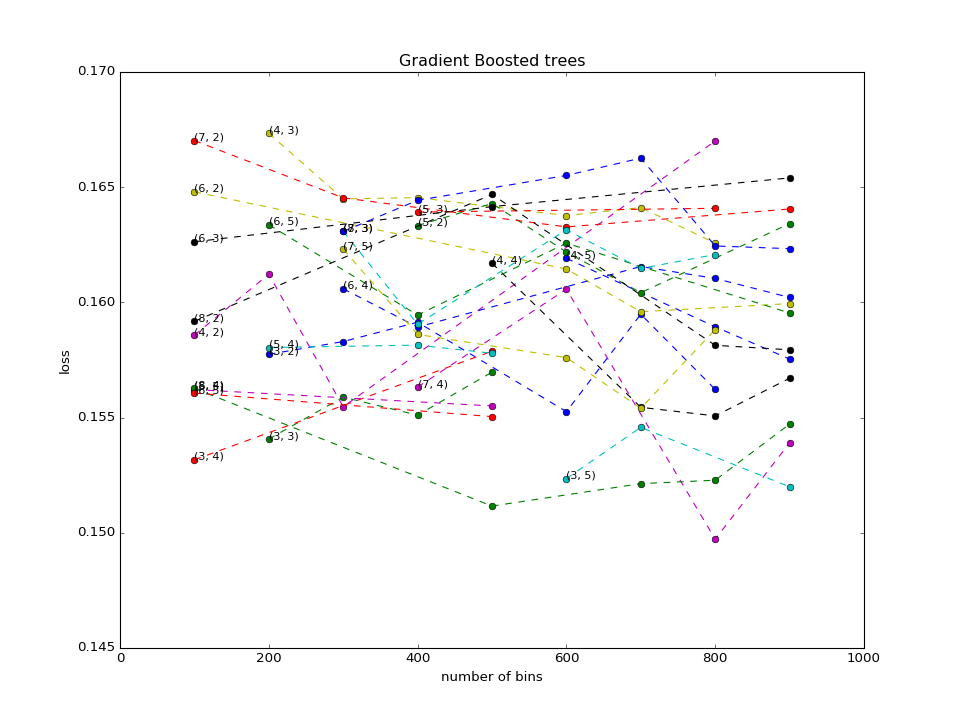
\includegraphics[width=0.6\linewidth]{xgb_loss_over_bins}
  \caption{Gradient Boosted trees average test sequence error as a function of $\protect n_{bins}$}
  \label{fig:xgb_loss_over_bins}
\end{figure}

Figures~\ref{fig:rf_loss_over_bins}, ~\ref{fig:xgb_loss_over_bins} are
rather crowded. We attempt a more concise and (possibly) clear version
of in Figures~\ref{fig:rf_average_loss_over_bins},
~\ref{fig:xgb_average_loss_over_bins}.  There we average losses for
each value of $n_{bins}$ over all available values of $n_x$ and $n_y$
(we also plot standard deviations as error bars).

A number of observations may be made based on these graphs:
\begin{itemize}
\item Gradient Boosting tends to outperform Random Forest.  This is an
  expected result.  Said that in our specific problem the gain is
  modest: the absolute average error of the gradient boosting is
  $10^{-2}$ order of magnitude outperforms the random forest.  Average
  scale magnitude is about $1m$, so we gain low single digit
  percentage advantage.
\item Standard deviation of losses is about $10^{-2}m$.  While being
  small, relative to mean scale magnitude, its significance should be
  evaluated in the context of motion estimation.  Small benefit in
  dead reconing may add up.
\item Best Random Forest regressor is $n_x=8$, $n_y=5$, $n_{bins}=500$ with loss of $0.1497 m$
\item Best Boosted Tree regressor is $n_x=7$, $n_y=4$, $n_{bins}=800$ with loss of $0.151 m$  
  
\end{itemize}

\begin{figure}[!ht]
  \centering  
  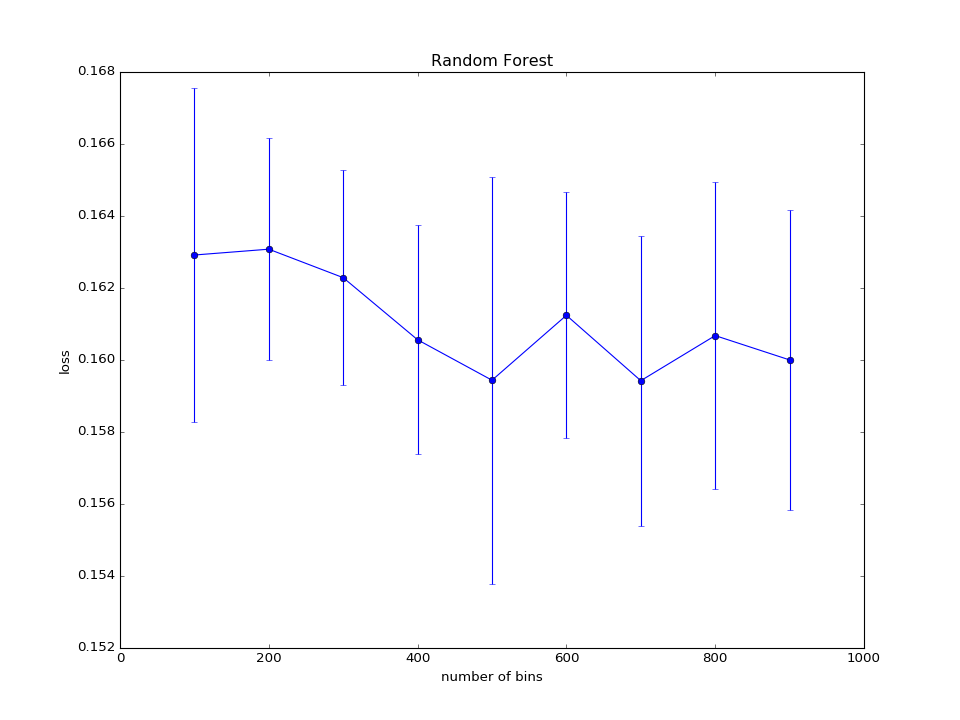
\includegraphics[width=0.6\linewidth]{rf_average_loss_over_bins}
  \caption{Random Forest trees average of average test sequence errors as a
    function of $\protect n_{bins}$}
  \label{fig:rf_average_loss_over_bins}
\end{figure}

\begin{figure}[!ht]
  \centering  
  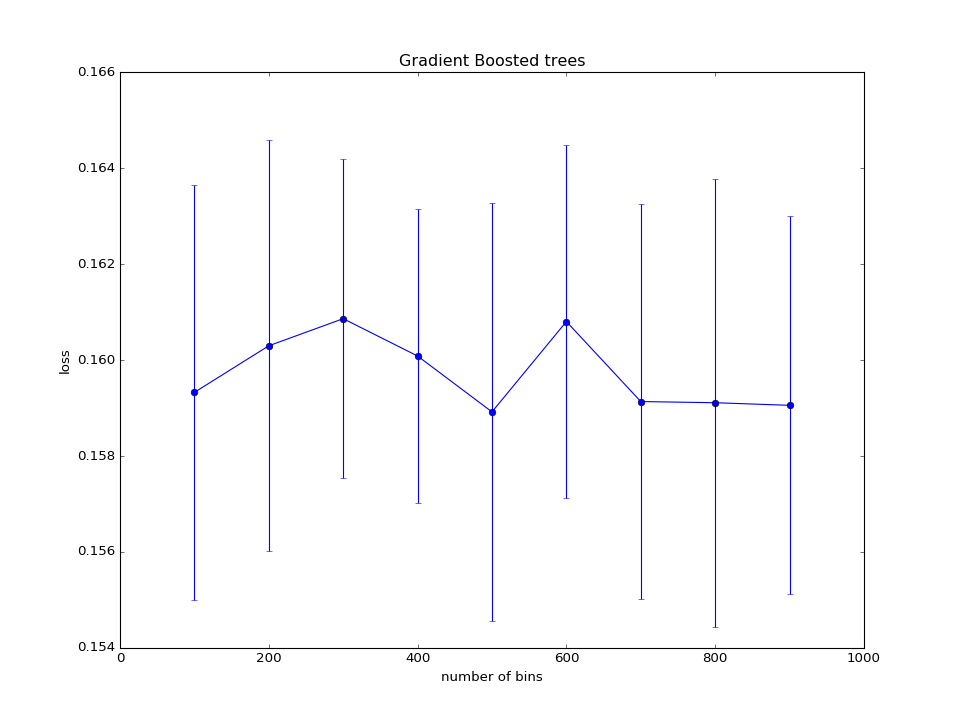
\includegraphics[width=0.6\linewidth]{xgb_average_loss_over_bins}
  \caption{Gradient Boosted trees average of average test sequence errors as a
    function of $\protect n_{bins}$}
  \label{fig:xgb_average_loss_over_bins}
\end{figure}

\section{Discussion}

\medskip

\bibliographystyle{unsrt}
\bibliography{report}

\end{document}

%%% Local Variables:
%%% mode: latex
%%% TeX-master: t
%%% End:
